\documentclass{article}

% Language setting
% Replace `english' with e.g. `spanish' to change the document language
\usepackage[english,greek]{babel}
\usepackage[utf8x]{inputenc}

% Set page size and margins
% Replace `letterpaper' with `a4paper' for UK/EU standard size
\usepackage[letterpaper,top=2cm,bottom=2cm,left=3cm,right=3cm,marginparwidth=1.75cm]{geometry}

% Useful packages
\usepackage{amsmath}
\usepackage{graphicx}
\usepackage[colorlinks=true, allcolors=blue]{hyperref}

\title{\textbf{Ανάπτυξη Εφαρμογής για Ανάλυση Δεδομένων}}

\author{\textbf{Μιχάλης Ζώης Π2010057}}
\date{}

\begin{document}
\maketitle
\thispagestyle{empty}
\begin{center}
    
\includegraphics[width=0.5\linewidth]{ionian_university.png}
\end{center}

\newpage
\tableofcontents
\setcounter{page}{1}
\newpage

\section{\selectlanguage{greek}Εισαγωγή}

Στην εποχή της πληροφορίας, η ικανότητα εξόρυξης και ανάλυσης δεδομένων αποτελεί κρίσιμο πλεονέκτημα για οργανισμούς και ερευνητές. Με την ανάπτυξη της τεχνολογίας, οι \selectlanguage{english}web-based \selectlanguage{greek}εφαρμογές προσφέρουν ευκολία και ευελιξία στη διαχείριση και ανάλυση μεγάλων συνόλων δεδομένων. Στην παρούσα εργασία, θα αναπτύξουμε μια τέτοια εφαρμογή χρησιμοποιώντας το \textbf{\selectlanguage{english}Streamlit}, \selectlanguage{greek}ένα ισχυρό εργαλείο για την ανάπτυξη διαδραστικών και δυναμικών \textbf{\selectlanguage{english}web-based} \selectlanguage{greek}εφαρμογών. 

\section{Στόχοι της Εφαρμογής}

Η εφαρμογή θα παρέχει τις ακόλουθες βασικές λειτουργίες:

\subsection{Φόρτωση Δεδομένων}

Η πρώτη βασική λειτουργία της εφαρμογής είναι η δυνατότητα φόρτωσης δεδομένων σε μορφή πίνακα \textbf{(\selectlanguage{english}tabular data)}, \selectlanguage{greek}όπως \textbf{\selectlanguage{english}CSV \selectlanguage{greek}ή \selectlanguage{english}Excel \selectlanguage{greek}}αρχεία. Τα δεδομένα θα πρέπει να οργανώνονται σε πίνακα με \selectlanguage{english}S \selectlanguage{greek}δείγματα και \selectlanguage{english}F \selectlanguage{greek} χαρακτηριστικά, με την τελευταία στήλη (\selectlanguage{english}F+1) \selectlanguage{greek}να περιέχει την ετικέτα (\selectlanguage{english}label) \selectlanguage{greek}για κάθε δείγμα.

\subsection{\selectlanguage{english}2D Visualization Tab}

Ένα από τα στοιχεία της εφαρμογής θα είναι το \selectlanguage{english}2D Visualization Tab. \selectlanguage{greek}Σε αυτό το τμήμα, οι χρήστες θα μπορούν να εκτελούν \selectlanguage{english}2D \selectlanguage{greek}οπτικοποιήσεις δεδομένων χρησιμοποιώντας δύο αλγορίθμους μείωσης διάστασης, όπως \textbf{\selectlanguage{english}PCA (Principal Component Analysis)} \selectlanguage{greek}και \textbf{\selectlanguage{english}t-SNE (t-Distributed Stochastic Neighbor Embedding)}. \selectlanguage{greek}Επιπλέον, θα παρουσιαστούν διαγράμματα για την διερευνητική ανάλυση δεδομένων \textbf{\selectlanguage{english}(Exploratory Data Analysis - EDA)}.

\subsection{\selectlanguage{english}Tabs \selectlanguage{greek}Μηχανικής Μάθησης}

\selectlanguage{greek}Η εφαρμογή διαθέτει δύο επιπλέον \selectlanguage{english}tabs, \selectlanguage{greek}το καθένα αφιερωμένο σε διαφορετικούς τύπους αλγορίθμων μηχανικής μάθησης:
\begin{itemize}
  \item \textbf{Κατηγοριοποίηση}: Σε αυτό το \selectlanguage{english}tab, \selectlanguage{greek}θα υλοποιηθούν και θα συγκριθούν δύο αλγόριθμοι κατηγοριοποίησης.
  \item \textbf{Ομαδοποίηση}: Σε αυτό το \selectlanguage{english}tab, \selectlanguage{greek}θα υλοποιηθούν και θα συγκριθούν δύο αλγόριθμοι ομαδοποίησης. Και σε αυτήν την περίπτωση, οι χρήστες θα μπορούν να καθορίσουν παραμέτρους όπως το \selectlanguage{english}'k' \selectlanguage{greek}στον αλγόριθμο \selectlanguage{english} k-means \selectlanguage{greek}και τα \selectlanguage{english}'eps', 'min-samples' \selectlanguage{greek}στον \selectlanguage{english}dbscan.
\end{itemize}

\newpage
\section{\selectlanguage{greek}Υλοποίηση και Αποτελέσματα}

\subsection{Αρχική σελίδα}

Στον χρήστη εμφανίζεται η επιλογή να ανεβάσει ένα αρχείο τύπου \textbf{\selectlanguage{english}CSV \selectlanguage{greek}ή \selectlanguage{english}Excel} \selectlanguage{greek}αρχείο.

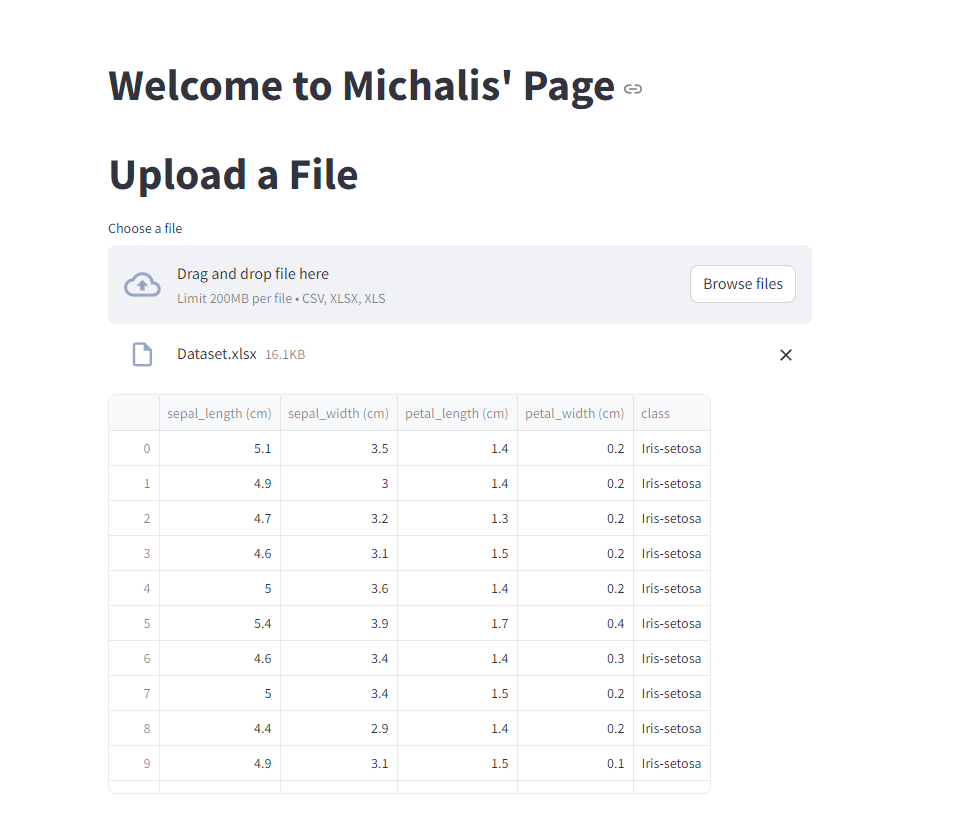
\includegraphics[width=1.0\linewidth]{home_page.png}
Μόλις ο χρήστης επιλέξει το αρχείο, τα δεδομένα εμφανίζονται στην σελίδα.

\subsection{\selectlanguage{english}2D Visualization Tab}

\selectlanguage{greek}Στην καρτέλα \selectlanguage{english}2D Visualization Tab \selectlanguage{greek}παρουσιάζονται σε διαγράμματα οι αλγόριθμοι \textbf{\selectlanguage{english}PCA, t-SNE, EDA}
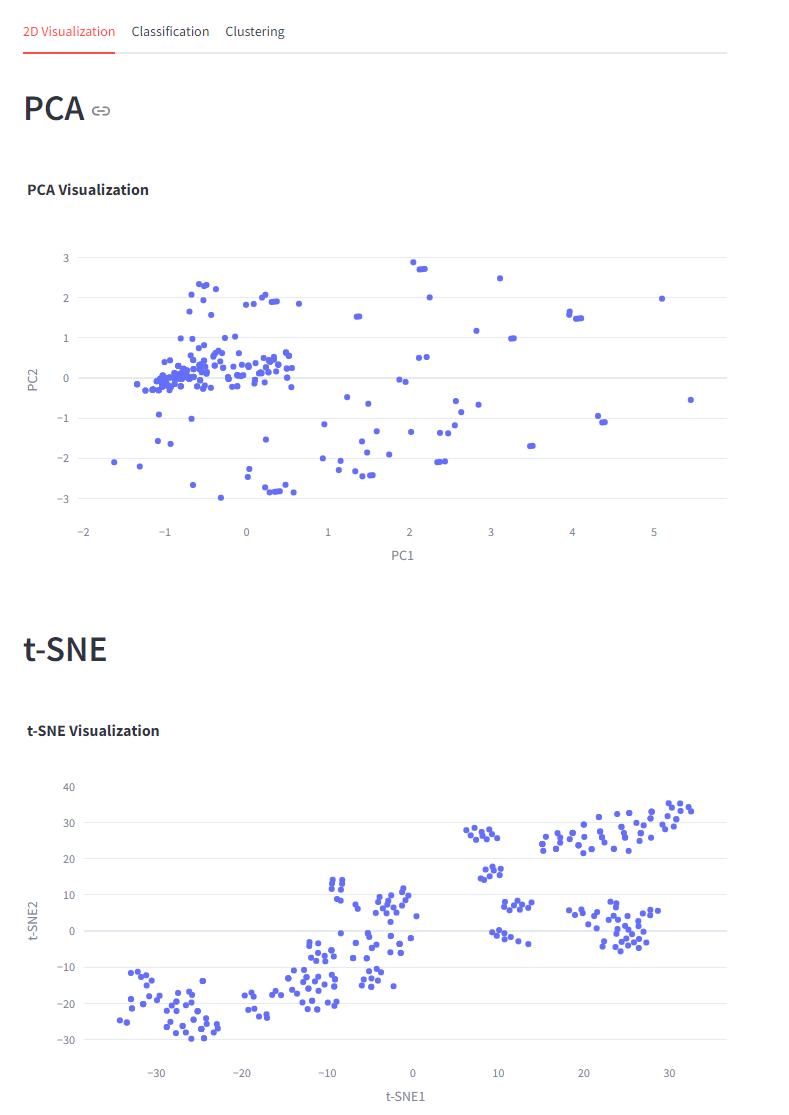
\includegraphics[width=1.0\linewidth]{tab0_pca_tsne1.png}
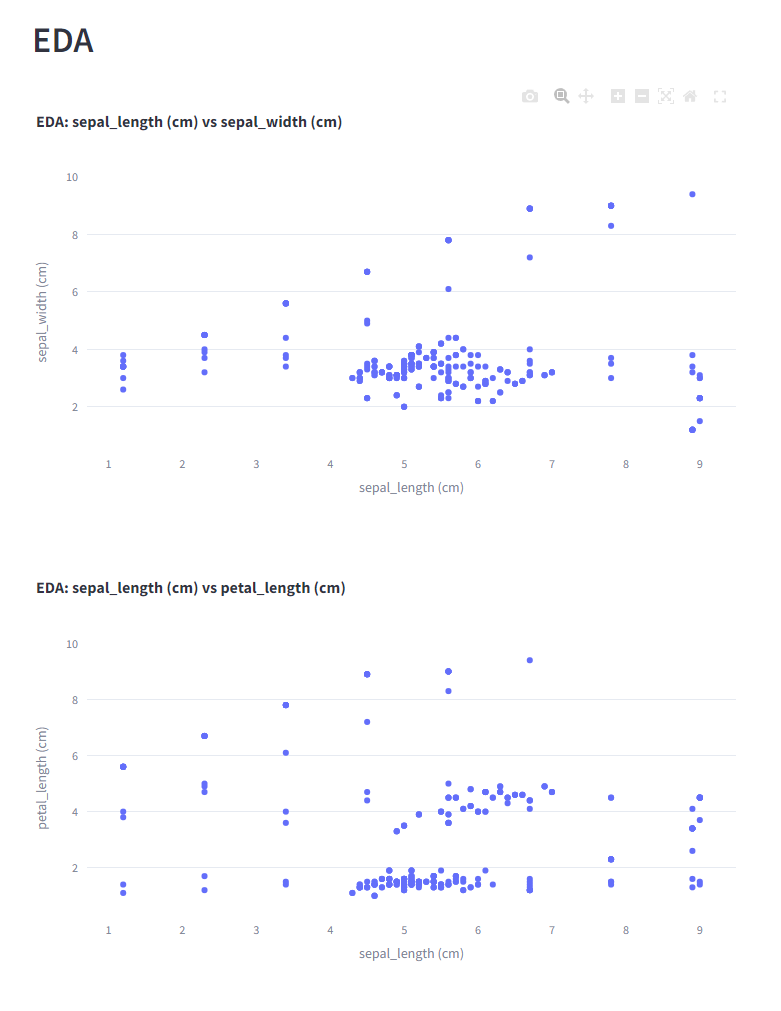
\includegraphics[width=1.0\linewidth]{tab0_eda1-2.png}
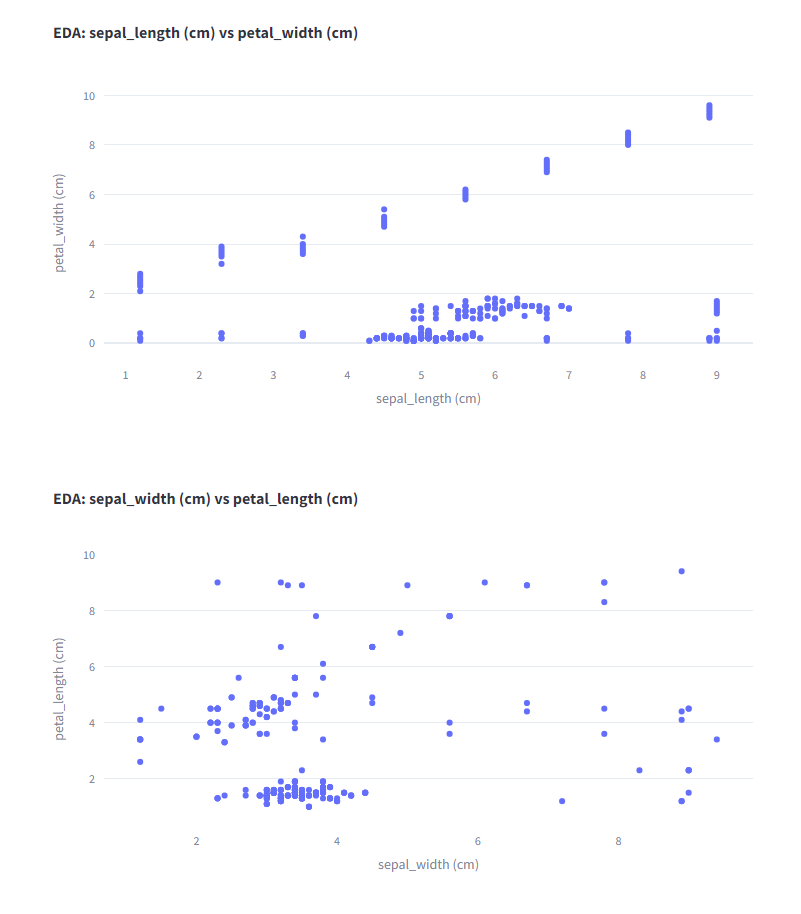
\includegraphics[width=1.0\linewidth]{tab0_eda3-4.png}
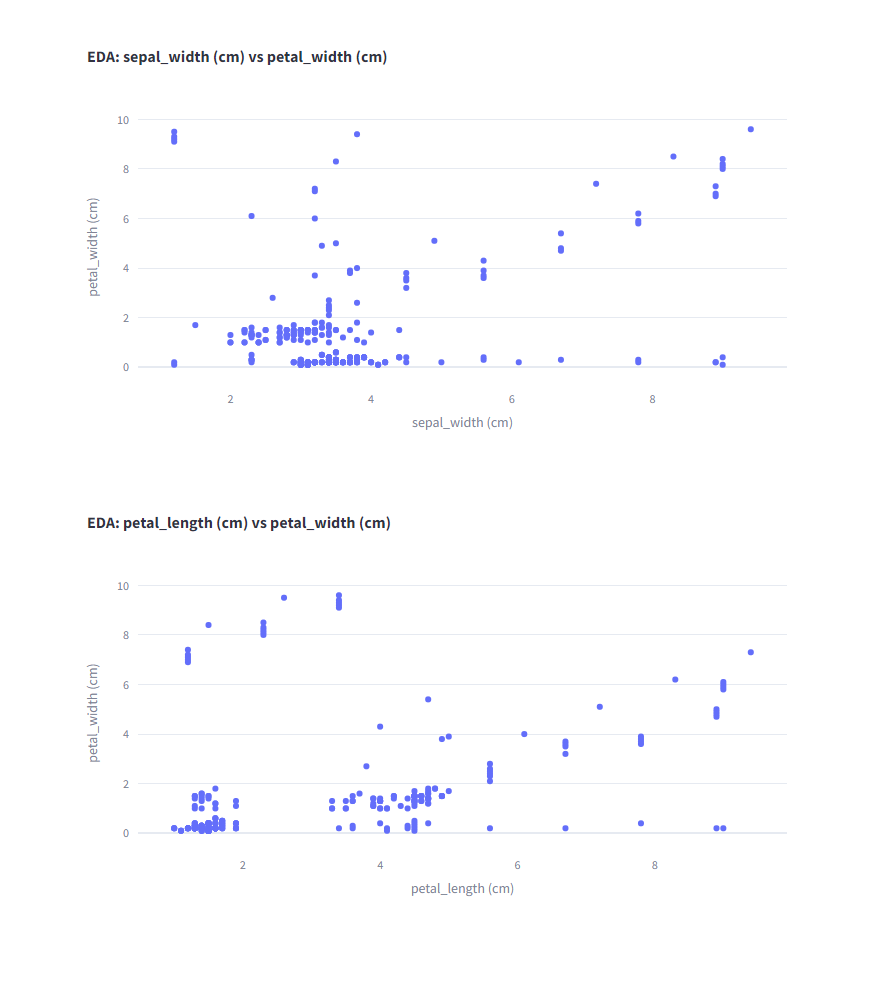
\includegraphics[width=1.0\linewidth]{tab0_eda5-6.png}

\subsection{\selectlanguage{english}Classification Tab}

\selectlanguage{greek} Στην καρτέλα \selectlanguage{english}Classification \selectlanguage{greek}παρουσιάζονται σε διαγράμματα οι αλγόριθμοι \textbf{\selectlanguage{english}Logistic Regression, SVM}
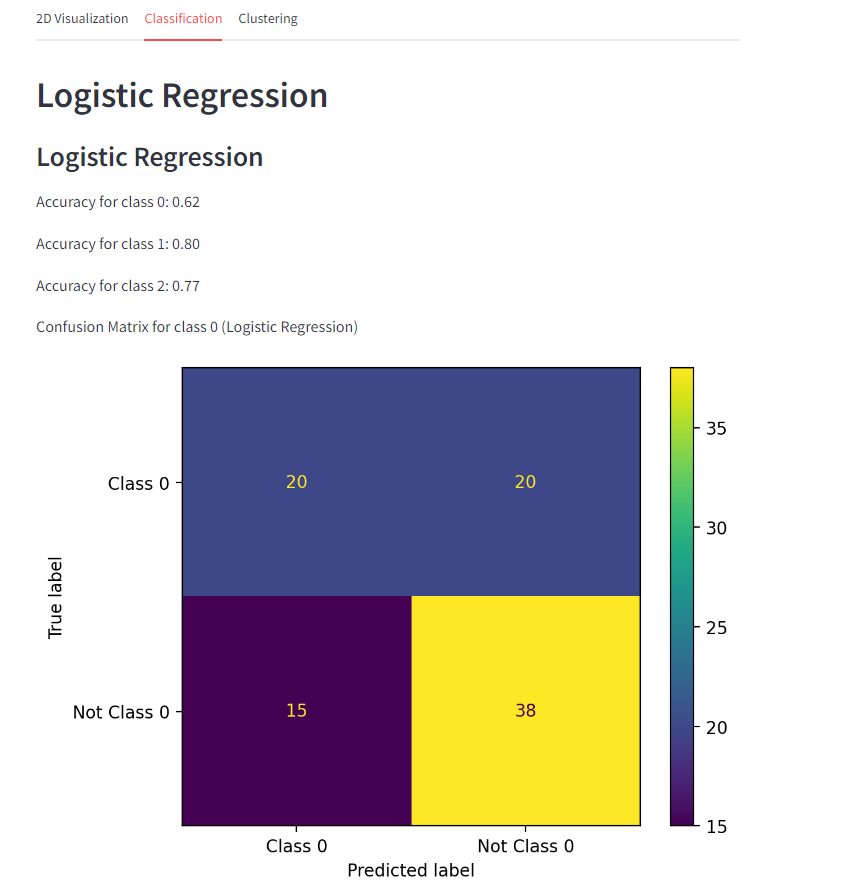
\includegraphics[width=1.0\linewidth]{tab1_logistic_regression1.png}
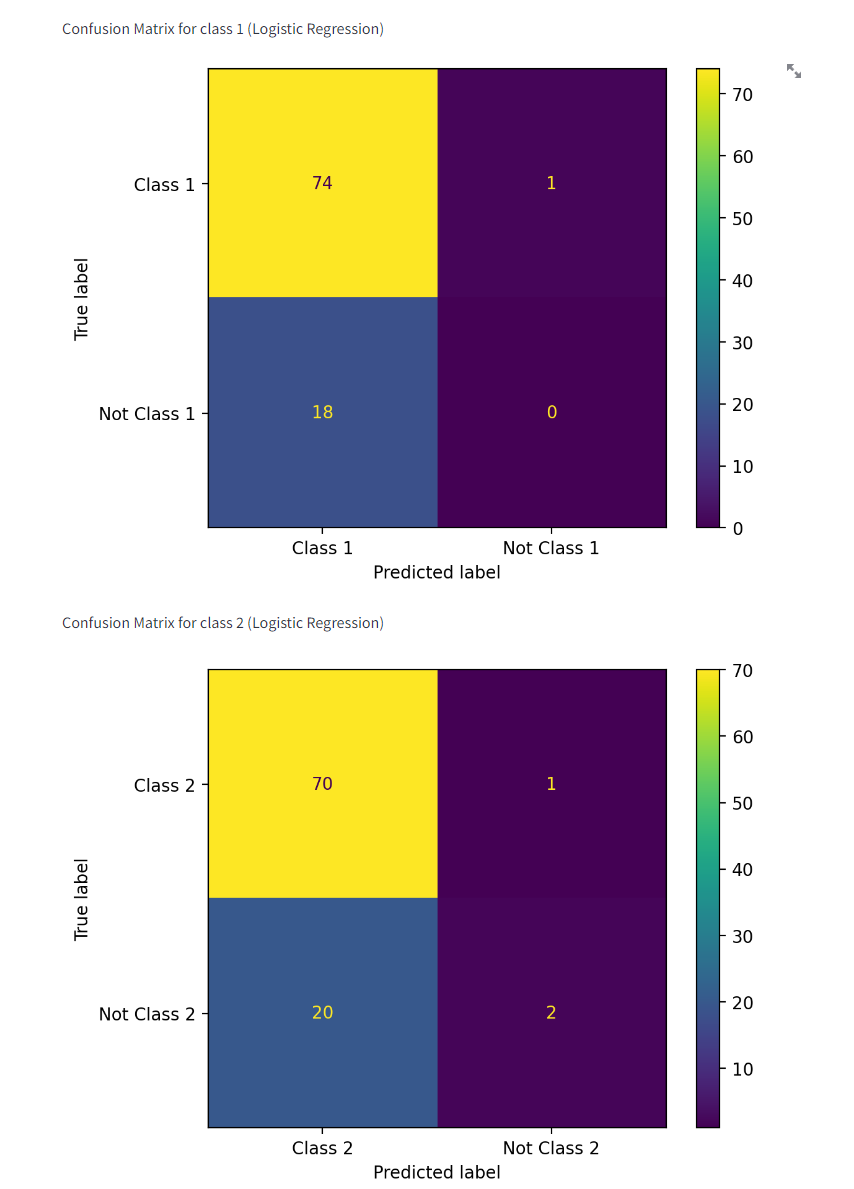
\includegraphics[width=1.0\linewidth]{tab1_logistic_regression2.png}
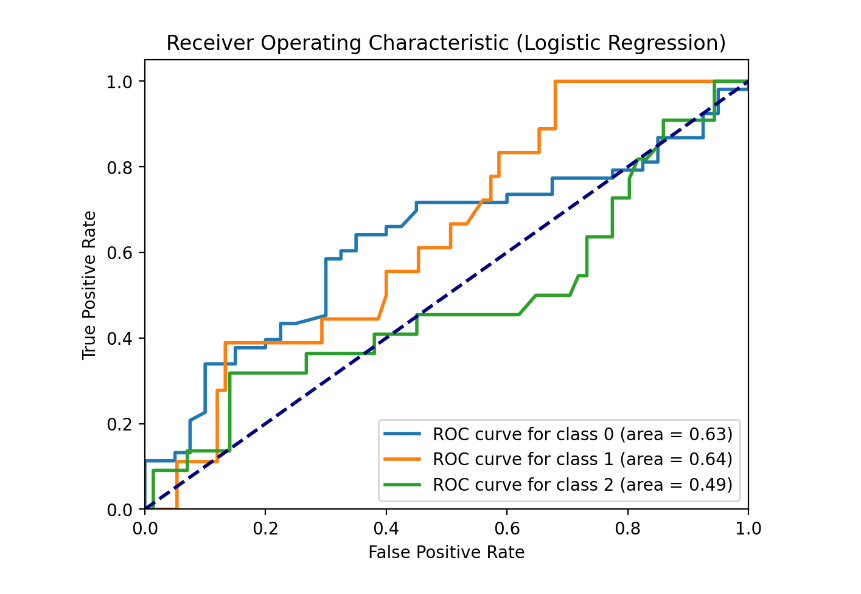
\includegraphics[width=1.0\linewidth]{tab1_logistic_regression3.png}

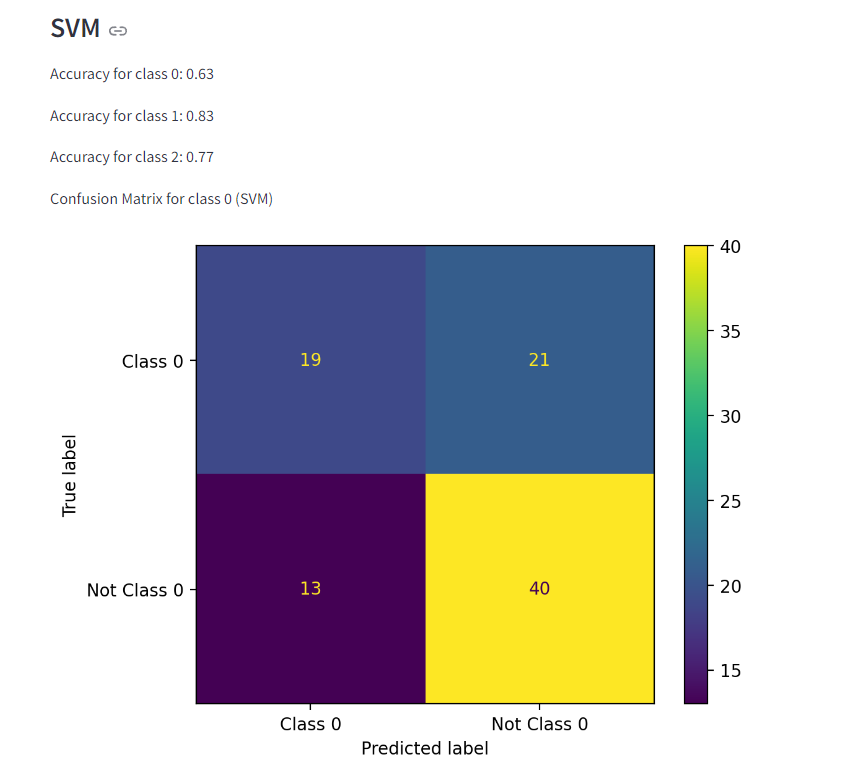
\includegraphics[width=1.0\linewidth]{tab1_svm1.png}
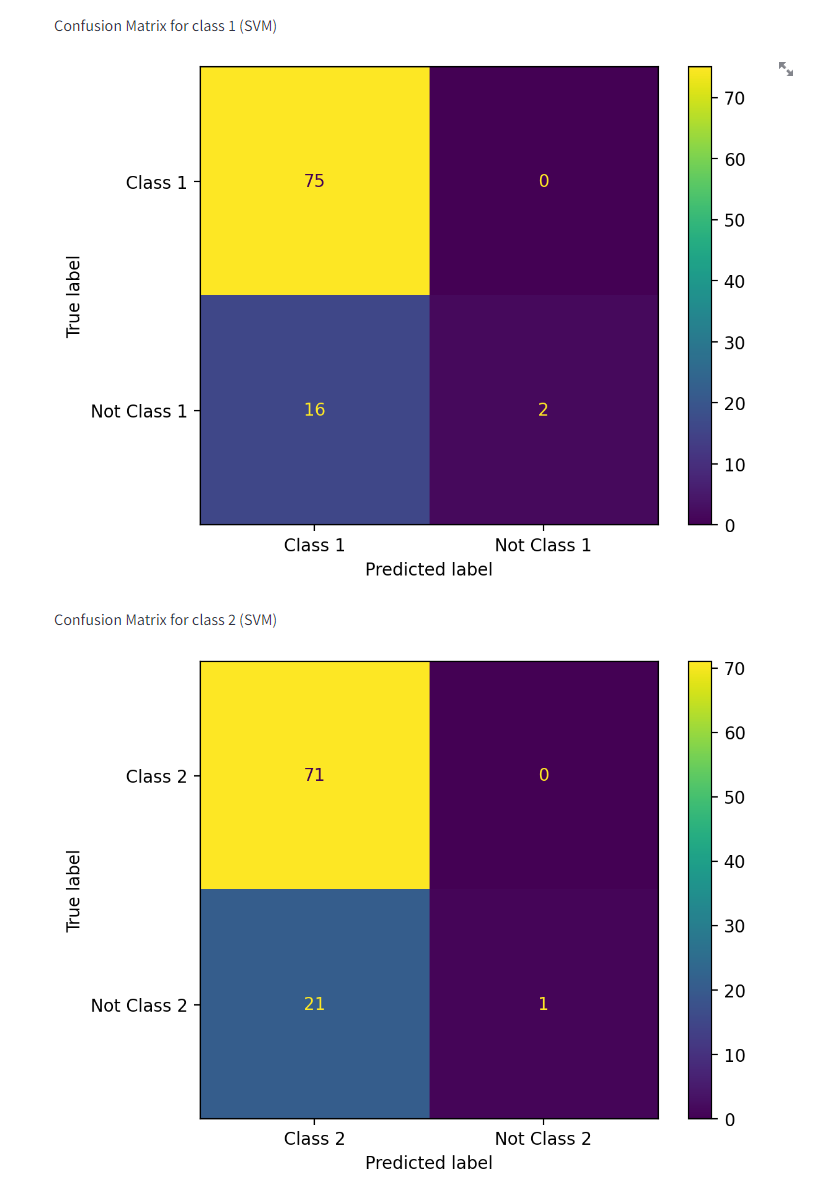
\includegraphics[width=1.0\linewidth]{tab1_svm2.png}
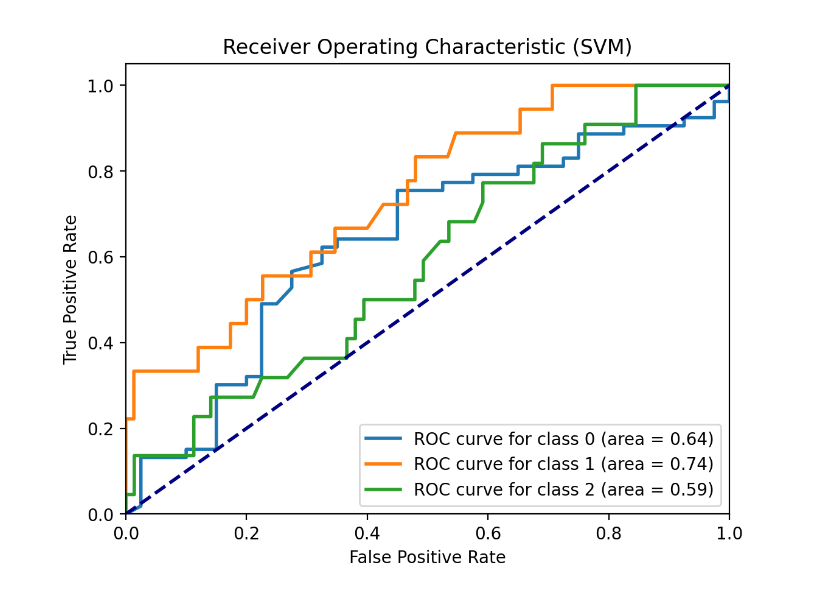
\includegraphics[width=1.0\linewidth]{tab1_svm3.png}

\newpage
\subsection{\selectlanguage{english}Clustering Tab}

\selectlanguage{greek} Στην καρτέλα \selectlanguage{english}Clustering \selectlanguage{greek}παρουσιάζονται σε διαγράμματα οι αλγόριθμοι \selectlanguage{english}k-means, DBScan.
\begin{itemize}
  \item \selectlanguage{greek}Στον αλγόριθμο \selectlanguage{english}k-means \selectlanguage{greek}ο χρήστης ορίζει τον αριθμό ομάδων \selectlanguage{english}'k'. \selectlanguage{greek}Ακολουθεί παράδειγμα με είσοδο το \selectlanguage{english}Dataset.xlsx \selectlanguage{greek}και \selectlanguage{english}'k=4'.
\end{itemize}

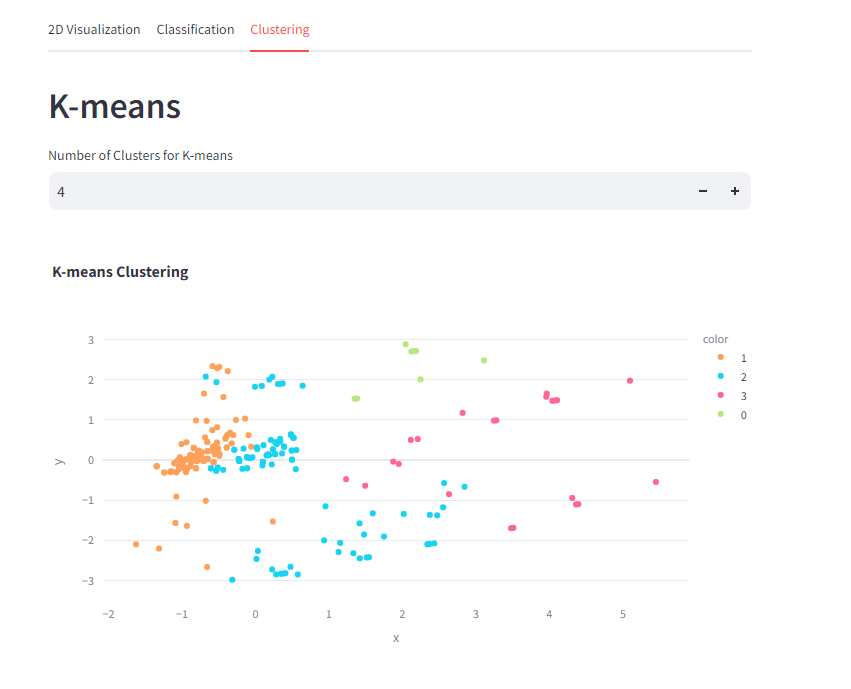
\includegraphics[width=1.0\linewidth]{tab2_kmeans.png}

\newpage
\begin{itemize}
  \item \selectlanguage{greek}Αντίστοιχα στον αλγόριθμο \selectlanguage{english}dbscan \selectlanguage{greek}ο χρήστης ορίζει το \selectlanguage{english}'eps' \selectlanguage{greek}και τoν ελάχιστο αριθμό δειγμάτων \selectlanguage{english}'min-samples'. \selectlanguage{greek}Ακολουθεί παράδειγμα με είσοδο το \selectlanguage{english}Dataset.xlsx \selectlanguage{greek}και \selectlanguage{english}'eps=0.30' - 'minimum samples=4'.
\end{itemize}

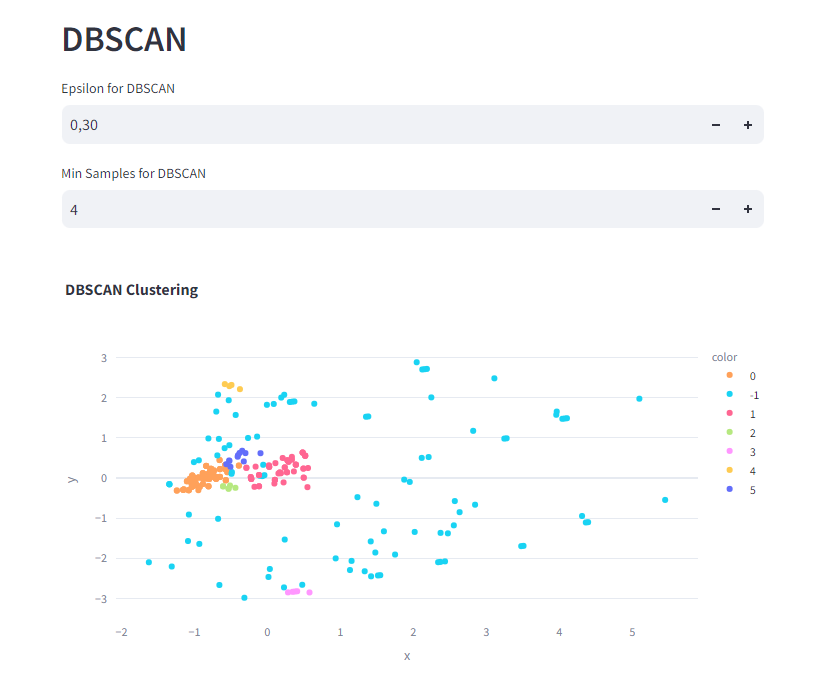
\includegraphics[width=1.0\linewidth]{tab2_dbscan.png}

\subsection{\selectlanguage{greek}Συμπεράσματα}
\begin{itemize}
  \item \textbf{\selectlanguage{english}PCA \selectlanguage{greek}και \selectlanguage{english}t-SNE}: \selectlanguage{greek}Τα δύο αυτά γραφήματα παρέχουν πολύτιμες απεικονίσεις της δομής των δεδομένων. Το \selectlanguage{english}t-SNE \selectlanguage{greek}δίνει καλύτερη τοπική απεικόνιση σε σχέση με το \selectlanguage{english}PCA, \selectlanguage{greek}καθιστώντας το ιδανικό για την ανάλυση της πυκνότητας των δεδομένων.
  \item \textbf{\selectlanguage{english}Logistic Regression vs SVM}: \selectlanguage{greek}Και οι δύο αλγόριθμοι έχουν καλή απόδοση, αλλά ο \selectlanguage{english}SVM \selectlanguage{greek}έχει πλεονέκτημα σε δεδομένα με μη γραμμικούς διαχωρισμούς λόγω της ευελιξίας του με τα \selectlanguage{english}kernels.
  \item \textbf{K-means vs DBSCAN}: \selectlanguage{greek}Ο \selectlanguage{english}K-means \selectlanguage{greek}είναι απλός και αποδοτικός για δεδομένα με σαφή διαχωρισμό σε κλάσεις, αλλά είναι ευαίσθητος σε εξωτερικές τιμές. Ο \selectlanguage{english}DBSCAN, \selectlanguage{greek}από την άλλη, είναι καλύτερος στον εντοπισμό πυκνών περιοχών και θορυβωδών σημείων, καθιστώντας τον ιδανικό για μη γραμμικές δομές.
\end{itemize}

\newpage
\subsection{\selectlanguage{english}Info Tab}
\selectlanguage{greek} Στην καρτέλα \selectlanguage{english}Info \selectlanguage{greek}παρουσιάζονται οι οδηγίες χρήσης της εφαρμογής.

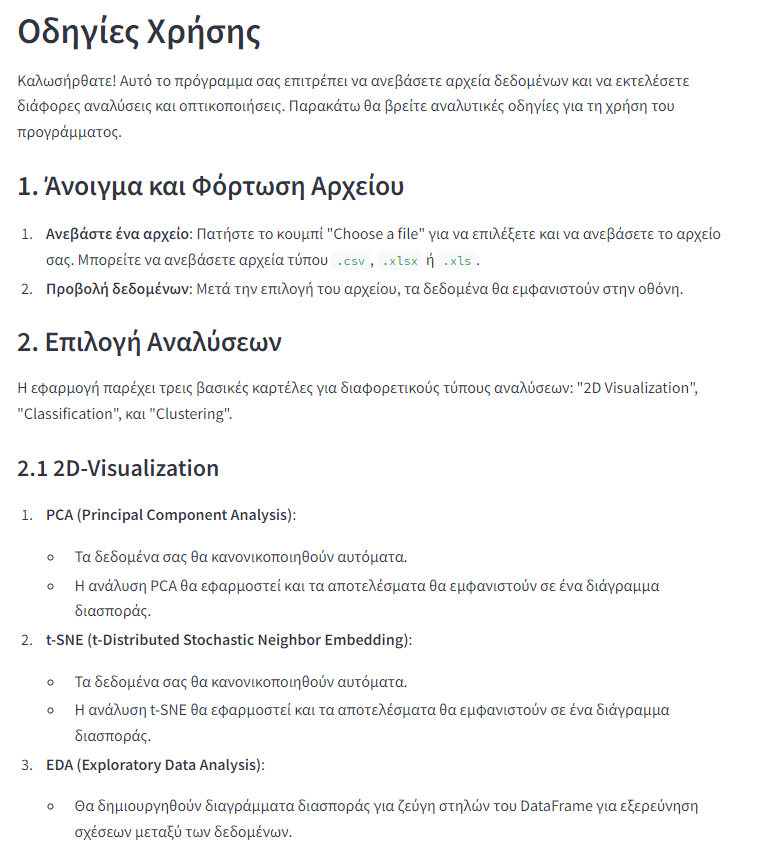
\includegraphics[width=1.0\linewidth]{tab3_info1.png}
\newpage
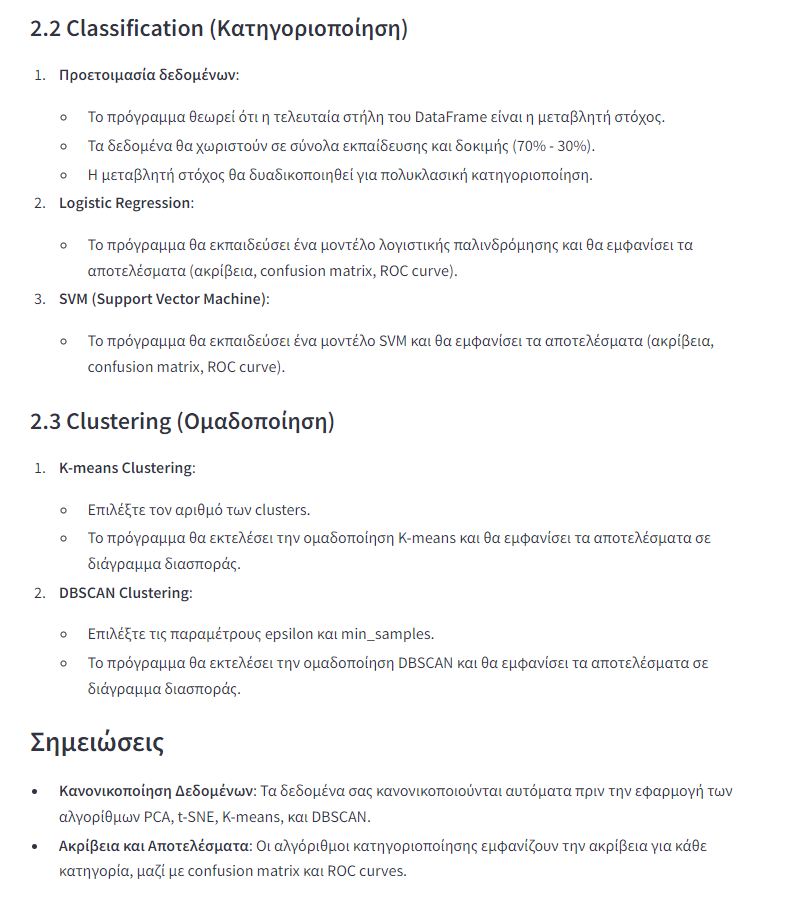
\includegraphics[width=1.0\linewidth]{tab3_info2.png}

\section{\selectlanguage{english}Uml \selectlanguage{greek}Διάγραμμα}
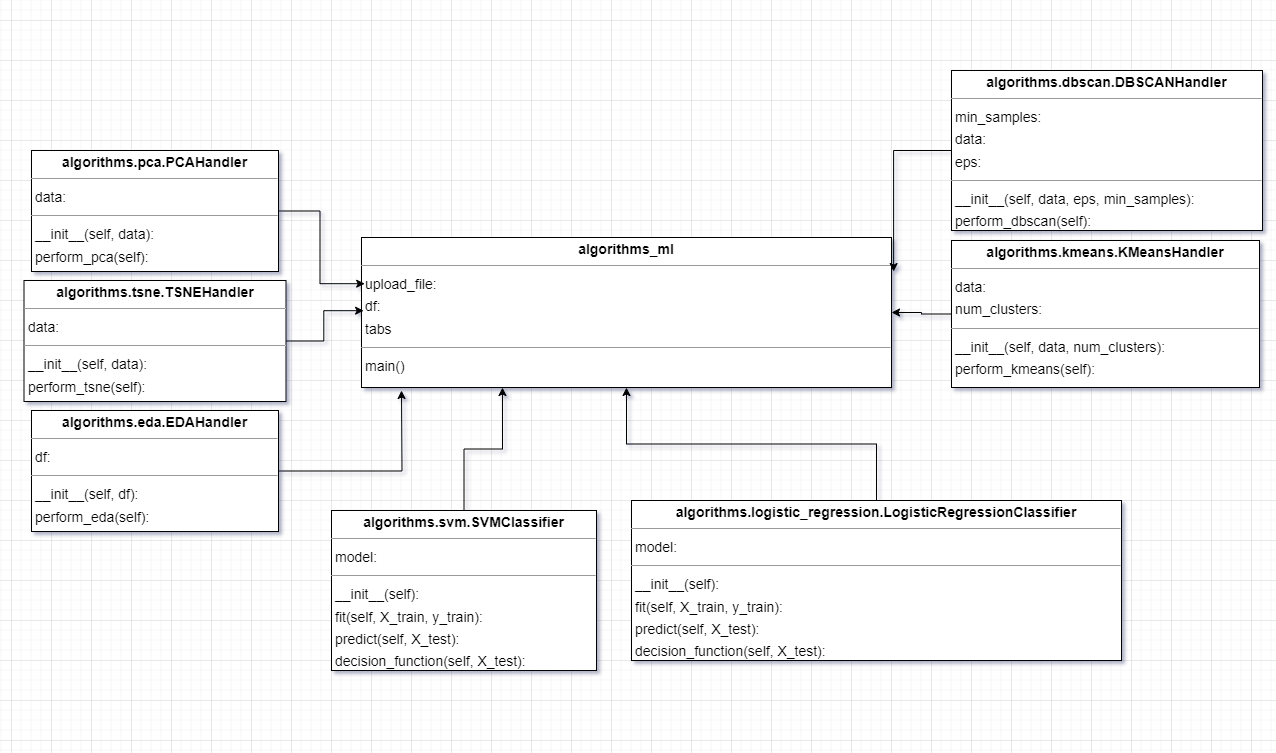
\includegraphics[width=1.0\linewidth]{uml_diagram.png}

\section{\selectlanguage{greek}Κύκλος Ζωής Έκδοσης Λογισμικού}
\selectlanguage{greek}Για την ανάπτυξη και διάθεση μιας εφαρμογής σε ευρύ κοινό, το \selectlanguage{english}Agile \selectlanguage{greek}μοντέλο λογισμικού είναι ιδιαίτερα αποτελεσματικό. Το \selectlanguage{english}Agile \selectlanguage{greek}είναι προσαρμόσιμο, επικεντρωμένο στον πελάτη και προσφέρει συνεχείς βελτιώσεις, κάνοντάς το ιδανικό για εφαρμογές που απευθύνονται σε μεγάλη και ποικιλόμορφη βάση χρηστών. Ακολουθεί μια περιγραφή του κύκλου ζωής της έκδοσης λογισμικού χρησιμοποιώντας το \selectlanguage{english}Agile \selectlanguage{greek}μοντέλο:
\subsection{\selectlanguage{greek}Αρχική Φάση: Σχεδιασμός και Οραματισμός}
\begin{itemize}
    \item \textbf{Ανάλυση Απαιτήσεων}: Συλλογή και ανάλυση των απαιτήσεων από τους χρήστες, τους ενδιαφερόμενους και την αγορά. Κατανόηση των αναγκών και των επιθυμιών του κοινού στόχου.
    \item \textbf{Οραματισμός Προϊόντος}: Δημιουργία του οράματος για την εφαρμογή, περιλαμβάνοντας τις βασικές λειτουργίες, τις αξίες που θα προσφέρει στους χρήστες και τα επιχειρησιακά οφέλη.
    \item \textbf{Χάρτης Πορείας (\selectlanguage{english}Roadmap)}: \selectlanguage{greek}Καθορισμός ενός χάρτη πορείας για την ανάπτυξη του προϊόντος με βασικά σημεία και στόχους.
\end{itemize}
% 

\subsection{Φάση Σχεδιασμού: Προετοιμασία και Κατανομή Εργασιών}
\begin{itemize}
    \item \textbf{\selectlanguage{english}Backlog \selectlanguage{greek}Δημιουργίας Προϊόντος}: Δημιουργία και ιεράρχηση ενός \selectlanguage{english}backlog \selectlanguage{greek}με όλα τα χαρακτηριστικά, τις βελτιώσεις και τις διορθώσεις σφαλμάτων που πρέπει να γίνουν.
    \item \textbf{\selectlanguage{english}Sprint Planning}: \selectlanguage{greek}Διαχωρισμός του έργου σε μικρότερες, διαχειρίσιμες ενότητες (\selectlanguage{english}sprints), \selectlanguage{greek}κάθε μία από τις οποίες έχει συγκεκριμένους στόχους και παραδοτέα.
\end{itemize}

\subsection{Φάση Ανάπτυξης: Επαναληπτικές και Συνεχείς Βελτιώσεις}
\begin{itemize}
    \item \textbf{Επαναληπτικές Κυκλοφορίες (\selectlanguage{english}Sprints)}: \selectlanguage{greek}Κάθε \selectlanguage{english}sprint \selectlanguage{greek}διαρκεί συνήθως 2-4 εβδομάδες. Περιλαμβάνει σχεδιασμό, ανάπτυξη, δοκιμή και αναθεώρηση των χαρακτηριστικών.
    \item \textbf{Καθημερινές Συναντήσεις (\selectlanguage{english}Daily Standups)}: \selectlanguage{greek}Καθημερινές σύντομες συναντήσεις για την ανασκόπηση της προόδου, την αντιμετώπιση προβλημάτων και την προσαρμογή των σχεδίων.
    \item \textbf{Ανασκοπήσεις και Αναδρομές (\selectlanguage{english}Sprint Reviews and Retrospectives)}: \selectlanguage{greek}Στο τέλος κάθε \selectlanguage{english}sprint, \selectlanguage{greek}γίνεται ανασκόπηση των αποτελεσμάτων και αναδρομή για τη βελτίωση των διαδικασιών.
\end{itemize}

\subsection{Φάση Δοκιμών: Εξασφάλιση Ποιότητας και Σταθερότητας}
\begin{itemize}
    \item \textbf{Συνεχής Ενσωμάτωση (\selectlanguage{english}Continuous Integration)}: \selectlanguage{greek}Καθημερινή ενσωμάτωση του κώδικα σε ένα κεντρικό αποθετήριο και εκτέλεση αυτοματοποιημένων δοκιμών για την ανίχνευση προβλημάτων νωρίς.
    \item \textbf{Δοκιμές Συστημάτων και Αποδοχής (\selectlanguage{english}System and Acceptance Testing)}: \selectlanguage{greek}Εκτενείς δοκιμές για τη διασφάλιση ότι η εφαρμογή λειτουργεί όπως αναμένεται σε διάφορα περιβάλλοντα και σενάρια χρήσης.
\end{itemize}

\subsection{Φάση Διάθεσης: Κυκλοφορία και Ανάδραση}
\begin{itemize}
    \item \textbf{Προετοιμασία για Κυκλοφορία (\selectlanguage{english}Release Planning)}: \selectlanguage{greek}Σχεδιασμός της κυκλοφορίας της εφαρμογής, περιλαμβάνοντας την επικοινωνία με τους χρήστες, την εκπαίδευση και την υποστήριξη.
    \item \textbf{Κυκλοφορία (\selectlanguage{english}Release)}: \selectlanguage{greek}Διαθεσιμότητα της εφαρμογής στο κοινό μέσω διαφόρων πλατφορμών (π.χ. \selectlanguage{english}App Store, Google Play, Web).
    \item \textbf{\selectlanguage{greek}Συλλογή Αναδράσεων (\selectlanguage{english}Feedback Gathering)}: \selectlanguage{greek}Συλλογή αναδράσεων από τους χρήστες και ανάλυση για την ταυτοποίηση ευκαιριών βελτίωσης και επίλυση προβλημάτων.
\end{itemize}

\subsection{Φάση Συντήρησης: Συνεχής Βελτίωση και Υποστήριξη}
\begin{itemize}
    \item \textbf{Διαχείριση Σφαλμάτων και Βελτιώσεων}: Συνεχής παρακολούθηση της εφαρμογής για σφάλματα και ευκαιρίες βελτίωσης, και γρήγορη ανταπόκριση σε αναδυόμενα ζητήματα.
    \item \textbf{Κυκλικές Αναβαθμίσεις (\selectlanguage{english}Iterative Upgrades)}: \selectlanguage{greek}Κυκλικές αναβαθμίσεις της εφαρμογής με νέα χαρακτηριστικά, βελτιώσεις απόδοσης και ασφάλειας.
\end{itemize}

\subsection{Φάση Ανατροφοδότησης και Προσαρμογής}
\begin{itemize}
    \item \textbf{Αναλύσεις Χρήσης (\selectlanguage{english}Usage Analytics)}: \selectlanguage{greek}Ανάλυση δεδομένων χρήσης για την κατανόηση των προτύπων χρήσης και την ταυτοποίηση περιοχών βελτίωσης.
    \item \textbf{Συνεχής Ανατροφοδότηση (\selectlanguage{english}Continuous Feedback Loop)}: \selectlanguage{greek}Συνεχής βελτίωση της εφαρμογής βασισμένη σε αναδράσεις χρηστών και αναλύσεις δεδομένων.
\end{itemize}

Το \textbf{\selectlanguage{english}Agile} \selectlanguage{greek}μοντέλο επιτρέπει την ευελιξία, την ταχεία ανταπόκριση στις αλλαγές και τη συνεχή βελτίωση, καθιστώντας το ιδανικό για την ανάπτυξη λογισμικού που προορίζεται για ευρεία διαθεσιμότητα και χρήση.
% 
\section{\selectlanguage{english}Github}
\selectlanguage{greek}Tο \textbf{\selectlanguage{english}Readme.md} \selectlanguage{greek}περιλαμβάνει το \textbf{'ονοματεπώνυμο'} και το \textbf{'ΑΜ'} \selectlanguage{greek}.
\newline
\href{https://github.com/mikezois1992/algorithms_ml}{\textbf{\selectlanguage{english}Link to github repository}} \selectlanguage{greek}(Κώδικας, \selectlanguage{english}Dockerfile, Dataset, Latex)

\end{document}